

\tikzset{every picture/.style={line width=0.75pt}} %set default line width to 0.75pt        

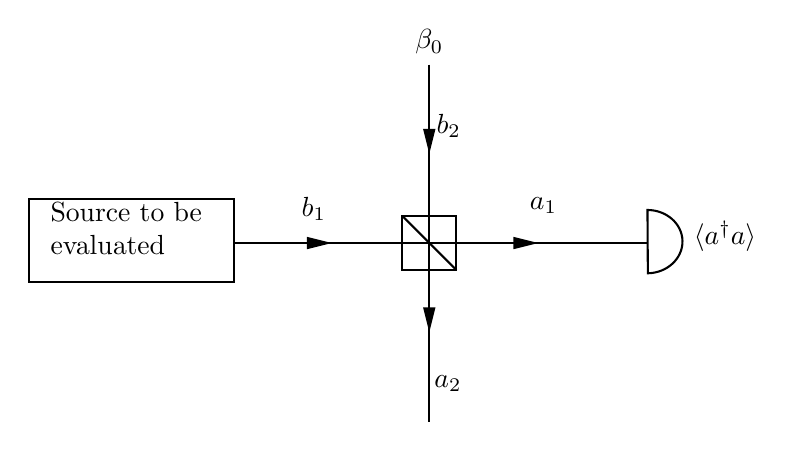
\begin{tikzpicture}[x=0.75pt,y=0.75pt,yscale=-1,xscale=1]
%uncomment if require: \path (0,300); %set diagram left start at 0, and has height of 300

%Straight Lines [id:da828543766930488] 
\draw    (228,144) -- (322,144) ;
\draw [shift={(275,144)}, rotate = 180] [fill={rgb, 255:red, 0; green, 0; blue, 0 }  ][line width=0.08]  [draw opacity=0] (12,-3) -- (0,0) -- (12,3) -- cycle    ;
%Shape: Square [id:dp6034028374707234] 
\draw   (335,131) -- (309,131) -- (309,157) -- (335,157) -- cycle ;
%Straight Lines [id:da08340572984807304] 
\draw    (335,157) -- (309,131) ;

%Straight Lines [id:da08559705327208378] 
\draw    (322,58) -- (322,144) ;
\draw [shift={(322,101)}, rotate = 270] [fill={rgb, 255:red, 0; green, 0; blue, 0 }  ][line width=0.08]  [draw opacity=0] (12,-3) -- (0,0) -- (12,3) -- cycle    ;
%Straight Lines [id:da571324279939923] 
\draw    (322,144) -- (427,144) ;
\draw [shift={(374.5,144)}, rotate = 180] [fill={rgb, 255:red, 0; green, 0; blue, 0 }  ][line width=0.08]  [draw opacity=0] (12,-3) -- (0,0) -- (12,3) -- cycle    ;
%Shape: Chord [id:dp5477809121009893] 
\draw   (427.11,128.08) .. controls (436.31,128.1) and (443.82,134.7) .. (443.98,143) .. controls (444.14,151.42) and (436.68,158.4) .. (427.3,158.58) -- cycle ;
%Shape: Rectangle [id:dp5820030129707479] 
\draw   (129,123) -- (228,123) -- (228,163) -- (129,163) -- cycle ;
%Straight Lines [id:da3527058340560272] 
\draw    (322,144) -- (322,230) ;
\draw [shift={(322,187)}, rotate = 270] [fill={rgb, 255:red, 0; green, 0; blue, 0 }  ][line width=0.08]  [draw opacity=0] (12,-3) -- (0,0) -- (12,3) -- cycle    ;

% Text Node
\draw (138,123) node [anchor=north west][inner sep=0.75pt]   [align=left] {Source to be \\evaluated};
% Text Node
\draw (322,54.6) node [anchor=south] [inner sep=0.75pt]    {$\ket{\beta _{0}}$};
% Text Node
\draw (259,120.4) node [anchor=north west][inner sep=0.75pt]    {$b_{1}$};
% Text Node
\draw (324,80.4) node [anchor=north west][inner sep=0.75pt]    {$b_{2}$};
% Text Node
\draw (323,206.4) node [anchor=north west][inner sep=0.75pt]    {$a_{2}$};
% Text Node
\draw (369,120.4) node [anchor=north west][inner sep=0.75pt]    {$a_{1}$};
% Text Node
\draw (448,140.7) node [anchor=west] [inner sep=0.75pt]    {$\langle a^{\dagger } a\rangle $};


\end{tikzpicture}
